\chapter{Arhitektura i dizajn sustava}
		
		%\textbf{\textit{dio 1. revizije}}\\

		%\textit{ Potrebno je opisati stil arhitekture te identificirati: podsustave, preslikavanje na radnu platformu, spremišta podataka, mrežne protokole, globalni upravljački tok i sklopovsko-programske zahtjeve. Po točkama razraditi i popratiti odgovarajućim skicama:}
	%\begin{itemize}
		%\item 	\textit{izbor arhitekture temeljem principa oblikovanja pokazanih na predavanjima (objasniti zašto ste baš odabrali takvu arhitekturu)}
		%\item 	\textit{organizaciju sustava s najviše razine apstrakcije (npr. klijent-poslužitelj, baza podataka, datotečni sustav, grafičko sučelje)}
		%\item 	\textit{organizaciju aplikacije (npr. slojevi frontend i backend, MVC arhitektura) }		
	%\end{itemize}

	
		Arhitektura sustava oblikovana je tako da se sastoji od tri podsustava:
		
		\begin{itemize}
			\item Web preglednik
			\item Web poslužitelj
			\item Baza podataka
		\end{itemize}
		
		\textbf{Web preglednik} služi korisniku za pristup poslužitelju i podacima u bazi podataka. To je program kojim korisnik može slati zahtjeve do poslužitelja za neku uslugu, u obliku dohvaćanja ili slanja podataka do poslužitelja. Web poslužitelj će nakon primitka zahtjeva od korisnika kroz Web preglednik prikazati odgovor na zahtjev. Dakle, Web preglednik je prvi korak za krajnjeg korisnika u interakciji sa sustavom u cjelini.
		
		
		\textbf{Web poslužitelj} je središnja komponenta sustava gdje se događaju svi važni izračuni te strukturiranje odgovora korisniku, a isto tako i pristup bazi podataka. To je program na jednom ili više računala, odnosno poslužitelja, koji interagira s jednim ili više korisnika. Zahtjeve prima preko HTTP protokola te vraća odgovor u obliku HTML dokumenta koji se prikazuje korisniku u njegovom Web pregledniku, potrebne podatke pohranjuje i ažurira u bazi podataka.
		
		
		\textbf{Baza podataka} je podsustav koji služi za pohranu svih potrebnih podataka. Backend strana Web aplikacije pristupa joj te upravlja podacima. Zbog učestalosti pristupa podacima u bazi podataka, od velike je važnosti da ona radi brzo i efikasno te je stoga bitno bazu podataka oblikovati efikasno i normalizirano.\\
		
		
		U izgradnji sustava koristi se objektno orijentirana paradigma. Za ovaj sustav to je programski jezik Java te radni okvir Spring koji je korišten za izradu backenda. Za izradu frontend dijela sustava, odnosno Web aplikacije upotrebljava se programski jezik JavaScript te biblioteka React. Uz to, za vanjsku komunikaciju kao pomoć u radu aplikacije, koristi se vanjski rječnik uz pomoć aplikacijskog sučelja.\\

				
		\section{Baza podataka}
			
			%\textbf{\textit{dio 1. revizije}}\\
			
		%\textit{Potrebno je opisati koju vrstu i implementaciju baze podataka ste odabrali, glavne komponente od kojih se sastoji i slično.}
		
Za potrebe rada sustava kojeg gradimo koristit ćemo relacijsku bazu podataka čiji su glavni elementi relacije. Relacije možemo promatrati kao tablice definirane svojim imenom te atributima. Relacijski model nastao je na temelju ER modela baze podataka čiji su temeljni elementi entiteti i veze. Zadatak baze podataka je brzo, kompaktno te jednostavno pohranjivanje, izmjenu te uklanjanje raznih podataka. Za ovaj sustav, to su podaci o korisničkim računima, podaci o pohranjenim rječnicima te riječima u njima, opisi riječi te stadij učenja u kojem se nalazi korisnik sustava. U skladu s tim, definiramo bazu podataka sastavljenu od entiteta:
			
			\begin{packed_item}
				
				\item Racun
				\item VrstaRacuna
				\item TrenutnoStanje
				\item Posuda
				\item ModUcenja
				\item Rjecnik
				\item Jezik
				\item Fraza
				\item Rijec
				\item rijecURjecniku
				\item rijecUPosudi
				
			\end{packed_item}
		
			\subsection{Opis tablica}
			

%				\textit{Svaku tablicu je potrebno opisati po zadanom predlošku. Lijevo se nalazi točno ime varijable u bazi podataka, u sredini se nalazi tip podataka, a desno se nalazi opis varijable. Svjetlozelenom bojom označite primarni ključ. Svjetlo plavom označite strani ključ}
				
				
				\textbf{Racun} Ovaj entitet sadrži informacije o korisničkom računu. Njegovi atributi su: idRacun, emailRacun, imeOsoba, prezimeOsoba, lozinkaRacun te idVrstaRacun. Ovaj entitet u vezi \textit{Many-to-One} je s entitetom VrstaRacuna preko atributa idVrstaRacun, u vezi \textit{One-to-Many} s entitetom Posuda preko atributa idRacun te u vezi \textit{One-to-Many} s entitetom TrenutnoStanje preko atributa idRacun.
				
				\begin{longtblr}[
					label=racun,
					entry=none
					]{
						width = \textwidth,
						colspec={|X[6,l]|X[6, l]|X[20, l]|}, 
						rowhead = 1,
					} %definicija širine tablice, širine stupaca, poravnanje i broja redaka naslova tablice
					\hline \SetCell[c=3]{c}{\textbf{Racun}}	 \\ \hline[3pt]
					\SetCell{LightGreen}idRacun & INT	&  	Jedinstven identifikator korisnika generiran od strane baze podataka (surogatni ključ)  	\\ \hline
					emailRacun	& VARCHAR &   Jedinstvena adresa elektroničke pošte (alternativni ključ)	\\ \hline 
					imeOsoba & VARCHAR & Ime korisnika  \\ \hline 
					prezimeOsoba & VARCHAR	&  	Prezime korisnika	\\ \hline 
					lozinkaRacun & VARCHAR & Kriptirana lozinka korisnika  \\ \hline
					\SetCell{LightBlue} idVrstaRacun	& INT &   Identifikator vrste računa korisnika	\\ \hline 
				\end{longtblr}
				
				\textbf{VrstaRacuna} Ovaj entitet sadrži informacije o vrsti korisničkog računa (radi li se o učeniku ili administratoru riječi). Njegovi atributi su: idVrstaRacun te imeVrstaRacun. Ovaj entitet u vezi \textit{One-to-Many} je s entitetom Racun preko atributa idVrstaRacun.
				
				\begin{longtblr}[
					label=vrstaRacuna,
					entry=none
					]{
						width = \textwidth,
						colspec={|X[7,l]|X[6, l]|X[19, l]|}, 
						rowhead = 1,
					} %definicija širine tablice, širine stupaca, poravnanje i broja redaka naslova tablice
					\hline \SetCell[c=3]{c}{\textbf{VrstaRacuna}}	 \\ \hline[3pt]
					\SetCell{LightGreen}idVrstaRacun & INT	&  Jedinstven identifikator vrste računa generiran od strane baze podataka (surogatni ključ)  	\\ \hline
					imeVrstaRacun	& VARCHAR &   Ime vrste računa	\\ \hline  
				\end{longtblr}
				
				\textbf{TrenutnoStanje} Ovaj slabi entitet sadrži informacije o trenutnom stanju u kojem se nalazi korisnik sustava. Njegovi atributi su: idRjecnik, idRacun, idModUcenja. Ovaj entitet u vezi \textit{Many-to-One} je s entitetom Rjecnik preko atributa idRjecnik, u vezi \textit{Many-to-One} je s entitetom Racun preko atributa idRacun, u vezi \textit{Many-to-One} je s entitetom ModUcenja preko atributa idModUcenja.
				
				\begin{longtblr}[
					label=trenutnoStanje,
					entry=none
					]{
						width = \textwidth,
						colspec={|X[6,l]|X[6, l]|X[20, l]|}, 
						rowhead = 1,
					} %definicija širine tablice, širine stupaca, poravnanje i broja redaka naslova tablice
					\hline \SetCell[c=3]{c}{\textbf{TrenutnoStanje}}	 \\ \hline[3pt]
					\SetCell{LightGreen}idRjecnik & INT	&  	Jedinstven identifikator rječnika (strani ključ)	\\ \hline
					\SetCell{LightGreen}idRacun & INT	&  	Jedinstven identifikator računa (strani ključ)	\\ \hline
					\SetCell{LightGreen}idModUcenja & INT	&  	Jedinstven identifikator moda (strani ključ) učenja 	\\ \hline
				\end{longtblr}
				
				\textbf{Posuda} Ovaj slabi entitet sadrži informacije o pojedinoj posudi riječi pridruženoj nekom korisniku. Njegovi atributi su: idPosuda, idRacun, vrijemeTrajanja, brojPosuda. Ovaj entitet u vezi \textit{Many-to-One} je s entitetom Racun preko atributa idRacun, u vezi \textit{Many-to-Many} je s entitetom Rijec preko atributa idRijec, idPosuda, idRacun.
				
				\begin{longtblr}[
					label=posuda,
					entry=none
					]{
						width = \textwidth,
						colspec={|X[7,l]|X[6, l]|X[19, l]|}, 
						rowhead = 1,
					} %definicija širine tablice, širine stupaca, poravnanje i broja redaka naslova tablice
					\hline \SetCell[c=3]{c}{\textbf{Posuda}}	 \\ \hline[3pt]
					\SetCell{LightGreen}idPosuda & INT	&  Jedinstveni identifikator posude riječi 	\\ \hline
					\SetCell{LightGreen}idRacun & INT & Jedinstveni identifikator računa korisnika (strani ključ) \\ \hline
					vrijemeTrajanja & INTERVAL & Vrijeme koje je potrebno proći kako bi se riječi iz posude pojavile u pitanju korisniku  \\ \hline 
					brojPosuda & INT	&  	Redni broj posude (alternativni ključ)	\\ \hline 
				\end{longtblr}
				
				\textbf{ModUcenja} Ovaj entitet sadrži informacije o modu učenja u kojem je korisnik. Njegovi atributi su: idModUcenja, opisModUcenja. Ovaj entitet u vezi \textit{One-to-Many} je s entitetom TrenutnoStanje preko atributa idModUcenja.
				
				\begin{longtblr}[
					label=modUcenja,
					entry=none
					]{
						width = \textwidth,
						colspec={|X[7,l]|X[6, l]|X[19, l]|}, 
						rowhead = 1,
					} %definicija širine tablice, širine stupaca, poravnanje i broja redaka naslova tablice
					\hline \SetCell[c=3]{c}{\textbf{ModUcenja}}	 \\ \hline[3pt]
					\SetCell{LightGreen}idModUcenja & INT	&  Jedinstven identifikator moda učenja generiran od strane baze podataka (surogatni ključ)  	\\ \hline
					opisModUcenja	& VARCHAR &   Kratki opis moda učenja	\\ \hline 
				\end{longtblr}
				
				\textbf{Rjecnik} Ovaj entitet sadrži informacije o rječniku za neki jezik. Njegovi atributi su: idRjecnik, imeRjecnik, idJezik. Ovaj entitet u vezi \textit{One-to-Many} je s entitetom TrenutnoStanje preko atributa idRjecnik, u vezi \textit{Many-to-One} s entitetom Jezik preko atributa idJezik te u vezi \textit{Many-to-Many} s entitetom Rijec preko atributa idRjecnik, idRijec.
				
				\begin{longtblr}[
					label=rjecnik,
					entry=none
					]{
						width = \textwidth,
						colspec={|X[6,l]|X[6, l]|X[20, l]|}, 
						rowhead = 1,
					} %definicija širine tablice, širine stupaca, poravnanje i broja redaka naslova tablice
					\hline \SetCell[c=3]{c}{\textbf{Rjecnik}}	 \\ \hline[3pt]
					\SetCell{LightGreen}idRjecnik & INT	&  	Jedinstveni identifikator rječnika generiran od strane baze podataka (surogatni ključ)  	\\ \hline
					imeRjecnik	& VARCHAR &   Ime rječnika	\\ \hline 
					\SetCell{LightBlue}idJezik	& INT &   Jedinstveni identifikator jezika kojem je rječnik pridružen	\\ \hline 
				\end{longtblr}
				
				\textbf{Jezik} Ovaj entitet sadrži informacije o jeziku kojeg podržava sustav. Njegovi atributi su: idJezik, kraticaJezik, imeJezik. Ovaj entitet u vezi \textit{One-to-Many} je s entitetom Rjecnik preko atributa idJezik.
				
				\begin{longtblr}[
					label=jezik,
					entry=none
					]{
						width = \textwidth,
						colspec={|X[6,l]|X[6, l]|X[20, l]|}, 
						rowhead = 1,
					} %definicija širine tablice, širine stupaca, poravnanje i broja redaka naslova tablice
					\hline \SetCell[c=3]{c}{\textbf{Jezik}}	 \\ \hline[3pt]
					\SetCell{LightGreen}idjezik & INT	&  Jedinstveni identifikator jezika generiran od strane baze podataka (surogatni ključ)	\\ \hline
					kraticaJezik	& CHAR &   Troslovna kratica jezika	\\ \hline 
					imeJezik & VARCHAR & Ime jezika  \\ \hline 
				\end{longtblr}
				
				\textbf{Fraza} Ovaj entitet sadrži informacije o frazi koja bolje opisuje neku riječ. Njegovi atributi su: idFraza, sadrzajFraza, idRijec. Ovaj entitet u vezi \textit{Many-to-One} je s entitetom Rijec preko atributa idRijec.
				
				\begin{longtblr}[
					label=fraza,
					entry=none
					]{
						width = \textwidth,
						colspec={|X[6,l]|X[6, l]|X[20, l]|}, 
						rowhead = 1,
					} %definicija širine tablice, širine stupaca, poravnanje i broja redaka naslova tablice
					\hline \SetCell[c=3]{c}{\textbf{Fraza}}	 \\ \hline[3pt]
					\SetCell{LightGreen}idFraza & INT	&  	Jedinstveni identifikator fraze generiran od strane baze podataka (surogatni ključ)  	\\ \hline
					sadrzajFraza	& VARCHAR &   Tekst fraze	\\ \hline 
					\SetCell{LightBlue}idRijec	& INT &   Jedinstveni identifikator riječi kojoj je fraza pridružena	\\ \hline 
				\end{longtblr}
				
				\textbf{Rijec} Ovaj entitet sadrži informacije o riječi koja je dodana u sustav. Njegovi atributi su: idRijec, sadrzajRijec, izgovorRijec. Ovaj entitet u vezi \textit{Many-to-Many} je s entitetom Posuda preko atributa idPosuda, idRijec, idRacun, u vezi \textit{Many-to-One} s entitetom Fraza preko atributa idFraza, u vezi je \textit{Many-to-Many} s entitetom Rjecnik preko atributa idRjecnik, idRijec.
				
				\begin{longtblr}[
					label=rijec,
					entry=none
					]{
						width = \textwidth,
						colspec={|X[6,l]|X[6, l]|X[20, l]|}, 
						rowhead = 1,
					} %definicija širine tablice, širine stupaca, poravnanje i broja redaka naslova tablice
					\hline \SetCell[c=3]{c}{\textbf{Rijec}}	 \\ \hline[3pt]
					\SetCell{LightGreen}idRijec & INT	&  Jedinstveni identifikator riječi generiran od strane baze podataka (surogatni ključ)	\\ \hline
					sadrzajRijec	& VARCHAR &   Sadržaj riječi	\\ \hline 
					izgovorRijec & BYTEA & Glasovna datoteka koja predstavlja izgovor riječi  \\ \hline 
				\end{longtblr}
				
				\textbf{rijecURjecniku} Ovaj entitet nastao zbog veze \textit{Many-to-Many} sadrži informacije o tome u kojim rječnicima se nalazi riječ. Njegovi atributi su: idRijec, idRjecnik.
				
				\begin{longtblr}[
					label=rijecURjecniku,
					entry=none
					]{
						width = \textwidth,
						colspec={|X[6,l]|X[6, l]|X[20, l]|}, 
						rowhead = 1,
					} %definicija širine tablice, širine stupaca, poravnanje i broja redaka naslova tablice
					\hline \SetCell[c=3]{c}{\textbf{rijecURjecniku}}	 \\ \hline[3pt]
					\SetCell{LightGreen}idRjecnik & INT	&  	Jedinstven identifikator rječnika (strani ključ)	\\ \hline
					\SetCell{LightGreen}idRijec & INT	&  	Jedinstven identifikator riječi (strani ključ)	\\ \hline
				\end{longtblr}
				
				\textbf{rijecUPosudi} Ovaj entitet nastao zbog veze \textit{Many-to-Many} sadrži informacije o u kojoj se posudi za koji račun nalazi neka riječ. Njegovi atributi su: idRijec, idPosuda, idRacun.
				
				\begin{longtblr}[
					label=rijecUPosudi,
					entry=none
					]{
						width = \textwidth,
						colspec={|X[6,l]|X[6, l]|X[20, l]|}, 
						rowhead = 1,
					} %definicija širine tablice, širine stupaca, poravnanje i broja redaka naslova tablice
					\hline \SetCell[c=3]{c}{\textbf{rijecUPosudi}}	 \\ \hline[3pt]
					\SetCell{LightGreen}idRijec & INT	&  	Jedinstven identifikator riječi (strani ključ)	\\ \hline
					\SetCell{LightGreen}idRacun & INT	&  	Jedinstven identifikator računa (strani ključ)	\\ \hline
					\SetCell{LightGreen}idPosuda & INT	&  	Jedinstven identifikator posude (strani ključ) učenja 	\\ \hline 
				\end{longtblr}
				
				
			
			\subsection{Dijagram baze podataka}
%				\textit{ U ovom potpoglavlju potrebno je umetnuti dijagram baze podataka. Primarni i strani ključevi moraju biti označeni, a tablice povezane. Bazu podataka je potrebno normalizirati. Podsjetite se kolegija "Baze podataka".}
			
%			\eject

				\begin{figure}[H]
					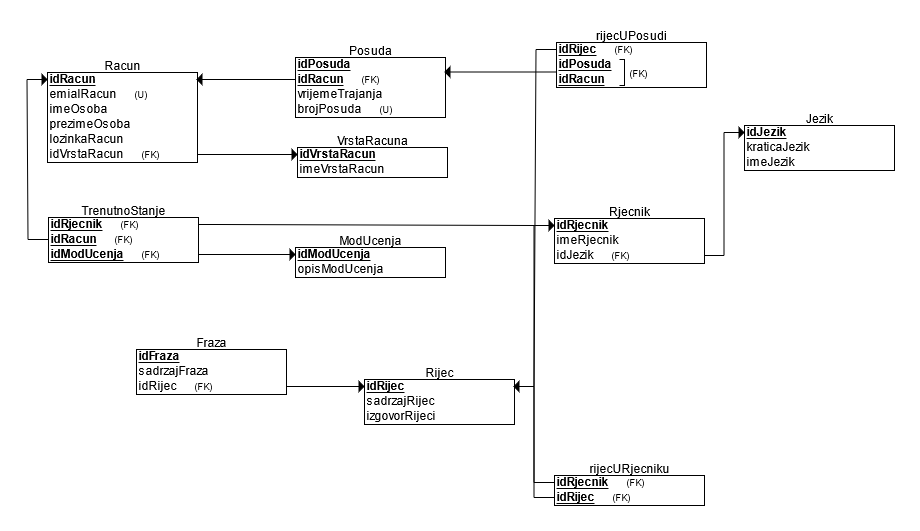
\includegraphics[width=\textwidth]{slike/dijagramBP.PNG}
					\caption{Dijagram baze podataka}
					\label{fig:dijagramBP}
				\end{figure}
			
			
		\section{Dijagram razreda}
		
			\textit{Potrebno je priložiti dijagram razreda s pripadajućim opisom. Zbog preglednosti je moguće dijagram razlomiti na više njih, ali moraju biti grupirani prema sličnim razinama apstrakcije i srodnim funkcionalnostima.}\\
			
			\textbf{\textit{dio 1. revizije}}\\
			
			\textit{Prilikom prve predaje projekta, potrebno je priložiti potpuno razrađen dijagram razreda vezan uz \textbf{generičku funkcionalnost} sustava. Ostale funkcionalnosti trebaju biti idejno razrađene u dijagramu sa sljedećim komponentama: nazivi razreda, nazivi metoda i vrste pristupa metodama (npr. javni, zaštićeni), nazivi atributa razreda, veze i odnosi između razreda.}\\
			
			\textbf{\textit{dio 2. revizije}}\\			
			
			\textit{Prilikom druge predaje projekta dijagram razreda i opisi moraju odgovarati stvarnom stanju implementacije}
			
			
			
			\eject
		
		\section{Dijagram stanja}
			
			
			\textbf{\textit{dio 2. revizije}}\\
			
			\textit{Potrebno je priložiti dijagram stanja i opisati ga. Dovoljan je jedan dijagram stanja koji prikazuje \textbf{značajan dio funkcionalnosti} sustava. Na primjer, stanja korisničkog sučelja i tijek korištenja neke ključne funkcionalnosti jesu značajan dio sustava, a registracija i prijava nisu. }
			
			
			\eject 
		
		\section{Dijagram aktivnosti}
			
			\textbf{\textit{dio 2. revizije}}\\
			
			 \textit{Potrebno je priložiti dijagram aktivnosti s pripadajućim opisom. Dijagram aktivnosti treba prikazivati značajan dio sustava.}
			
			\eject
		\section{Dijagram komponenti}
		
			\textbf{\textit{dio 2. revizije}}\\
		
			 \textit{Potrebno je priložiti dijagram komponenti s pripadajućim opisom. Dijagram komponenti treba prikazivati strukturu cijele aplikacije.}